\section{Interpretation of limits}
\label{sec:interpretation}

A light CP-odd Higgs boson ($m_A < 125$~GeV), which may or may not be related to global symmetries being present, exists in many extensions of the SM. Its couplings with gauge bosons are generically suppressed, yielding weak bounds from LEP. If $m_A<m_{h_{\rm SM}}/2$, it may be searched via the 
decay $h_{\rm SM} \to AA$. Though such decay sometimes has a large branching ratio, being in conflict with current Higgs precision data, there do exist scenarios, in both supersymmetric and non-supersymmetric theories, where the ${\cal B}(h_{\rm SM}\to AA)$ is suppressed. 
Therefore, new strategies for collider searches that could cover as large as possible model parameter space with a light CP-odd Higgs boson, are necessary. 
Next, we will interpret our collider analysis of $t\bar t A$ in several representative beyond-SM scenarios. 

\subsection{2HDM}

In the MSSM, a supersymmetric extension of a type-II 2HDM, a scenario with a light CP-odd Higgs boson is hard to achieve, given constraints from precision Higgs data. This is not surprising since there are only two free parameters at tree level in the Higgs sector, due to supersymmetric interrelations. The picture, however, is changed in the 2HDM without supersymmetry. With a softly-broken $Z_2$ symmetry ($\Phi_1 \to \Phi_1$, $\Phi_2 \to -\Phi_2$), which is often introduced to suppress scalar-mediated flavor changing processes, the Higgs potential of the 2HDM is given by: 
\begin{eqnarray} 
V(\Phi_1,\Phi_2) &=& m^2_1 \Phi^{\dagger}_1\Phi_1+m^2_2
\Phi^{\dagger}_2\Phi_2 + (m^2_{12} \Phi^{\dagger}_1\Phi_2+{\mathrm{h.c.}
}) +\frac{1}{2} \lambda_1 (\Phi^{\dagger}_1\Phi_1)^2 +\frac{1}{2}
\lambda_2 (\Phi^{\dagger}_2\Phi_2)^2\nonumber \\ 
&& +\lambda_3
(\Phi^{\dagger}_1\Phi_1)(\Phi^{\dagger}_2\Phi_2) + \lambda_4
(\Phi^{\dagger}_1\Phi_2)(\Phi^{\dagger}_2\Phi_1) + \frac{1}{2}
\lambda_5[(\Phi^{\dagger}_1\Phi_2)^2+{\mathrm{h.c.}}].
\end{eqnarray}
Here $\Phi_{1,2}$ are complex $SU(2)_L$ doublets. Assuming no CP-violation, the model has two CP-even and one CP-odd spin-0 neutral eigenstates, denoted as $h$, $H$, and $A$, respectively. Such a setup contains seven free parameters at tree level (including all Higgs masses), yielding a large parameter space that can accommodate a light CP-odd Higgs boson. 

Theoretically, the 125 GeV SM-like Higgs boson $h_{\rm SM}$ could be either the light CP-even Higgs boson ($h$) or the heavy one ($H$). If $m_A < m_{h_{\rm SM}}/2$, the decay $h_{\rm SM}\to AA$ is kinematically allowed. Often the partial width for $h_{\rm SM}\to AA$ becomes comparable or ever dominant over that of $h_{\rm SM}\to b\bar{b}$, given that the latter is suppressed by the lightness of the bottom quark.  Therefore, $h_{\rm SM} \to AA$ decays become a good probe for these light bosonic particles. However, as discussed recently~\cite{Bernon:2014nxa},\footnote{See Refs.~\cite{Draper:2010ew,Huang:2014cla} for discussions in the context of the NMSSM.} in the alignment limit [$\cos(\beta -\alpha)=0$ if $h_{\rm SM}=h$, and $\sin(\beta -\alpha)=0$ if $h_{\rm SM}=H$], which is favoured by current precision Higgs measurements, the Higgs coupling $g_{h_{\rm SM} AA}$ is reduced to: 
\begin{eqnarray}
\left|g_{h_{\rm SM} AA}\right | = \left |-\frac{2 m_A^2 + m_{h_{\rm SM}}^2  - 4 m_{12}^2/\sin 2\beta }{v}\right |.
\end{eqnarray}
In case that  $2 m_A^2 + m_{h_{\rm SM}}^2  \sim 4 m_{12}^2/\sin 2\beta$, the decay $h_{\rm SM}\to AA$ would be greatly suppressed. Therefore, collider strategies  are needed to probe these scenarios with $m_A < m_{\rm SM}/2$, as well as the scenarios with $m_A > m_{\rm SM}/2$.

We should note that the perturbation requirement for Higgs couplings yields bounds on $\tan\beta$. Particularly, the coupling $\lambda_1$ is related to the Higgs boson mass via the relation \cite{Bernon:2014nxa}: 
\begin{eqnarray}
\lambda_1 = \frac{m_h^2 + m_H^2 \tan^2\beta -  m_{12}^2 (\tan\beta +\tan^3 \beta)}{v^2}.
\end{eqnarray}
Assuming $g_{h_{\rm SM}\to AA}=0$, it becomes: 
\begin{eqnarray}
\lambda_1 = \frac{m_h^2 + \tan^2\beta (m_H^2 - m_{h_{\rm SM}}^2/2 - m_A^2)  }{v^2}.
\end{eqnarray}
Given $m_H^2 - m_{h_{\rm SM}}^2/2 - m_A^2 > 0$ for $m_A < m_{h_{\rm SM}}/2$, the perturbativity condition $\lambda_1 < 4\pi$ immediately sets an upper bound for $\tan\beta$ in this region:
\begin{eqnarray}
\tan\beta < \sqrt {\frac{4 \pi v^2 - m_h^2}{m_H^2 - m_{h_{\rm SM}}^2/2 - m_A^2 }} <  \sqrt {\frac{4 \pi v^2 }{m_{h_{\rm SM}}^2/2 - m_A^2 }}  \sim 10-20.
\end{eqnarray} 
These features are illustrated in Fig.~\ref{fig:Brhaa_2HDM}.  Additionally, the perturbation requirement for top Yukawa couplings can bound the $\tan\beta$ value from below. So we will limit our discussions for $\tan\beta > 0.1$. 

\begin{figure}[htbp]
\begin{center}
\begin{tabular}{c}
%   \\
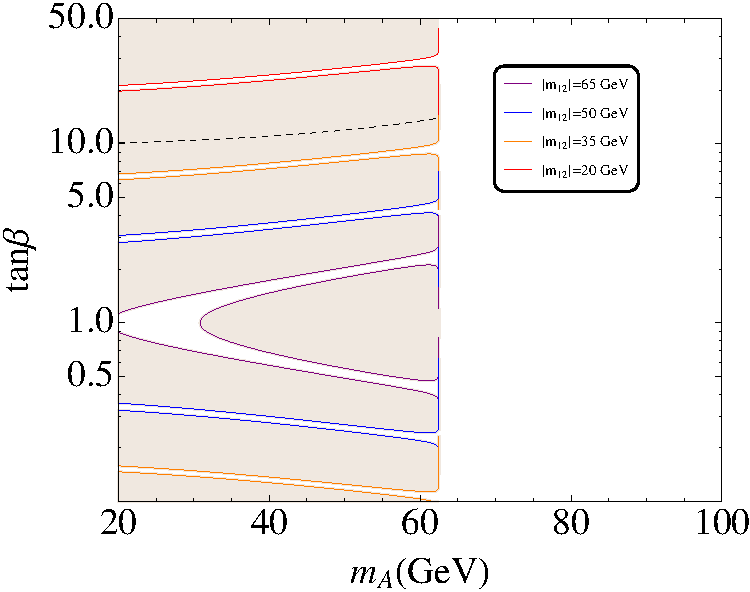
\includegraphics[width=0.5\textwidth]{Figures/pheno/plot_Brhaa_2HDM} 
\end{tabular}
\caption{Parameter region with ${\cal B}(h_{\rm SM}\to AA)<30\%$ in the 2HDM (blank region). The blank belts in the region with $m_A < m_{h_{\rm SM}}/2$, which are characterised by different boundary colours, are yielded by different $m_{12}^2$ values. The black dashed line represents a universal upper limit on $\tan\beta$ due to the perturbation requirement for $\lambda_1$.}
\label{fig:Brhaa_2HDM} 
\end{center}
\end{figure}


\begin{figure}[htbp]
\begin{center}
\begin{tabular}{cc}
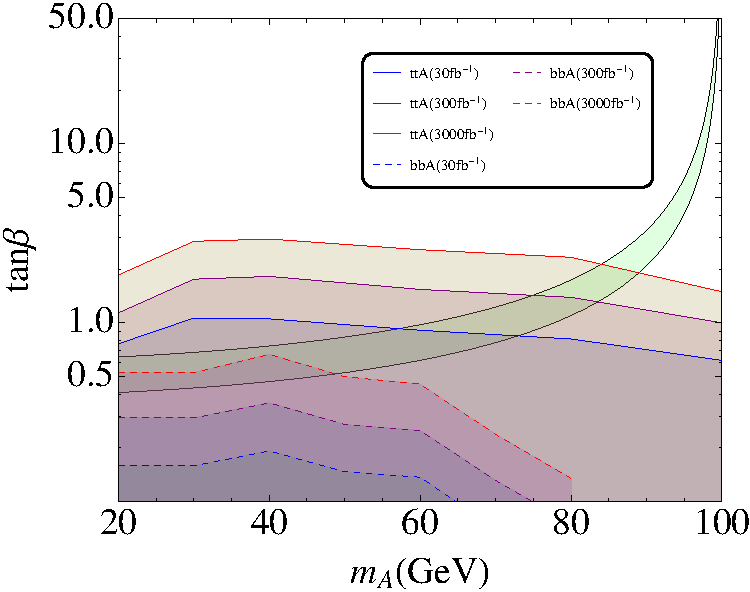
\includegraphics[width=0.45\textwidth]{Figures/pheno/plot_reach1_2HDM} &
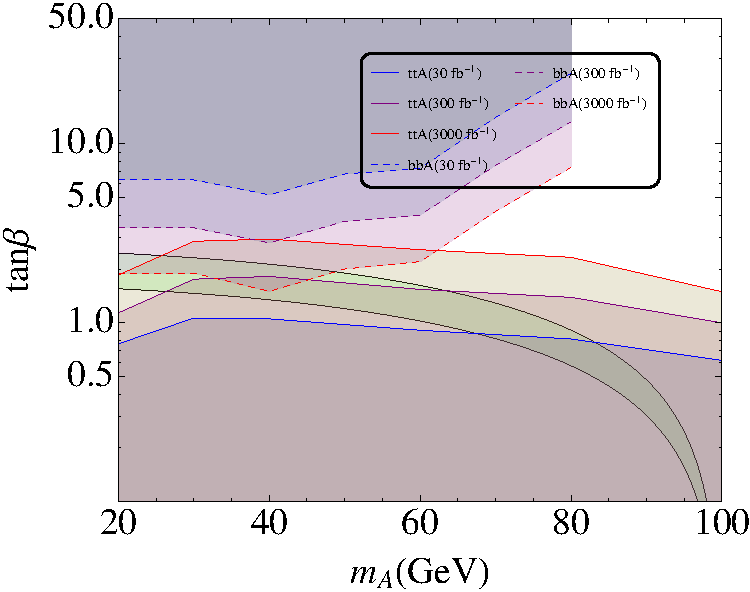
\includegraphics[width=0.45\textwidth]{Figures/pheno/plot_reach2_2HDM} \\
(a) & (b) \\
\end{tabular}
\caption{Sensitivity reach (at 95\% CL) of the $b\bar {b} A$ and $t\bar{t}A$ channels within the (a) type-I 2HDM and (b) type-II 2HDM. The green bands represent a region where the recently observed gamma-ray excess from the Galactic Centre can be explained, yielding a DM annihilation cross section of $\langle \sigma v \rangle  \simeq 1-2.5 \times 10^{-26} {\rm cm}^3 {\rm s}^{-1}$. Here the DM particle mass $m_{\chi}=50$~GeV and the coupling between the mediator and the DM particles $y_\chi= 0.3$ are assumed.  }
\label{fig:reach_2HDM} 
\end{center}
\end{figure}

The expected sensitivities for probing these scenarios in the 2HDM via $b\bar bA$ and $t\bar{t}A$ production are presented in Fig.~\ref{fig:reach_2HDM}. For illustration, we focus on type-I and type-II 2HDMs. The $b\bar{b}A$ reach is estimated based on the projections from Ref.~\cite{Kozaczuk:2015bea}, neglecting
systematic uncertainties. Within a type-II  2HDM, the $t\bar{t}A$ and $b\bar{b}A$ channels are complementary to each other in searching for light CP-odd Higgs bosons, since the coupling $g_{bbA}$ is $\tan\beta$-enhanced whereas $g_{ttA}$ is $\cot \beta$-enhanced. With integrated luminosities in excess of 300~fb$^{-1}$, the whole parameter region can be covered except a corner with relatively large $m_A$ and moderate $\tan\beta$. This is interesting given that low $\tan\beta$ is particularly favoured by perturbativity. In contrast, within a type-I 2HDM, the coupling $g_{bbA}$ would also be $\cot\beta$-enhanced, so both search channels are no longer probing complementary $\tan\beta$ regions. As a matter of fact, in such scenario the $t\bar{t}A$ channel provides a better sensitivity to search for the light CP-odd Higgs boson over the whole mass range of $20~{\rm GeV} < m_A < 100~{\rm GeV}$, although the high-$\tan\beta$ region remains difficult to probe. 

Searches for $t\bar {t}A$ and $b\bar {b} A$ also provide a probe for DM physics. For example, consider a Dirac fermion $\chi$ that is a DM candidate, with mass $m_\chi$, and coupling to the CP-odd scalar $A$ via:
\begin{eqnarray}
\mathcal {L} \supset y_\chi A \bar \chi i  \gamma^5 \chi.
\end{eqnarray}
Integrating out $A$ yields a dimension-six effective operator:
\begin{eqnarray}
\mathcal {L}_{\rm eff} \sim  \frac{- y_b y_\chi m_b   }{\Lambda^3} \bar \chi   \gamma^5 \chi \bar b   \gamma^5 b.
\end{eqnarray}
Such an operator implies s-wave DM annihilation $\chi \chi \to b\bar{b}$ with
\begin{equation}
\left < \sigma v \right > = \frac{3}{8 \pi} \frac{y^2_\chi g_b^2 y_b^2 m_{\chi}^2}{(m_A^2 - 4 m_{\chi}^2)^2 + m_A^2 \Gamma_A^2} \sqrt{1-\frac{m_b^2}{m_\chi^2}},
\label{eq:anhil}
\end{equation}
allowing an explanation for the recently observed diffuse gamma-ray excess from the Galactic Centre \cite{Goodenough:2009gk,Vitale:2009hr},  and a spin-dependent and p-wave-suppressed direct detection signal, resulting in a weak bound from current direct detection searches. In Fig.~\ref{fig:reach_2HDM}, the $\tan\beta$--$m_A$ values consistent with an explanation of the gamma-ray excess are indicated, yielding a DM annhilation cross section of $\langle \sigma v \rangle  \simeq 1-2.5 \times 10^{-26} {\rm cm}^3 {\rm} s^{-1}$, with $m_{\chi}=50$~GeV \cite{Calore:2014nla} and  $y_\chi= 0.3$ assumed.  
In this scenario, monojet searches at the LHC would also be insensitive since the decay $A \to \chi \chi$ would be kinematically forbidden, while the $t\bar {t}A$, $A \to b\bar{b}$ search would provide an effective probe.

\subsection{NMSSM}

Another class of benchmark scenairos for light CP-odd Higgs bosons arise in the NMSSM, with the superpotential and soft
supersymmetry-breaking terms of its Higgs sector given by
\begin{align}
\mathbf{W} &= \lambda \mathbf{S} \mathbf{H_u} \mathbf{H_d} + \frac{1}{3}\kappa {\bf S}^3, 
\nonumber \\
V_{\text{soft}} &= {m^2_{H_d}} |H_d|^2 + {m^2_{H_u}} |H_u|^2 + {m^2_S}|S|^2 - (\lambda A_{\lambda} H_u H_d S + \text{ h.c.} ) +  (\frac{1}{3} \kappa A_{\kappa} S^3 + \text{ h.c.} ),
\label{eqn:PQlimit}
\end{align}
where $H_d$, $H_u$ and $S$ denote the neutral Higgs fields of the ${\bf H_d}$, ${\bf H_u}$ and ${\bf S}$ supermultiplets, respectively. For convenience, let's define its CP-even and CP-odd mass eigenstates as $H_i$, $i=1,2,3$, and $A_j$, $j=1,2$, respectively.

In contrast with the 2HDM case, the light CP-odd Higgs boson in the NMSSM often results from breaking an approximate global symmetry spontaneously, serving as an axion or a pseudo-Goldstone boson. Its appearance is thus less ``artificial''. Let us start with the tree-level mass matrix of the CP-odd Higgs bosons in the NMSSM: 
\begin{eqnarray}
\mathcal{M}^2_{P} & = & \left(
\begin{array}{cc}
m_A^2
&\lambda  v \left(\frac{m_A^2 }{2\mu }\sin 2 \beta -\frac{3 \kappa  \mu }{\lambda }\right)
\\
%\lambda  v \left(\frac{\text{mA}^2 s_\beta c_\beta}{\mu }-\frac{3 \kappa  \mu }{\lambda }\right)
&
\lambda ^2 v^2 s_{2\beta}  \left(\frac{m_A^2}{4\mu ^2} \sin 2 \beta+\frac{3 \kappa }{2\lambda }\right)-\frac{3
   \kappa  A_{\kappa } \mu }{\lambda }\\
\end{array} 
\right), \ \  m_A^2 = \frac{2 \mu (A_\lambda + \kappa s) }{\sin 2 \beta} \nonumber\\
\end{eqnarray}
which yields a determinant
\begin{eqnarray}
\det(\mathcal{M}^2_{P}) = 9 \kappa \lambda v^2 \mu A_\lambda - \frac{6 A_\kappa \kappa \mu^2}{\lambda \sin2\beta} \left( A_\lambda + \frac{\kappa \mu }{\lambda} \right).
\end{eqnarray}
Necessarily, the scenarios with a light $A_1$ ($A_1$ denotes the lightest CP-odd Higgs boson) or $m_{A_1} \to 0$ yield $\det(\mathcal{M}^2_{P})  \to 0$
%\begin{eqnarray}
%\det(\mathcal{M}^2_{P})  \to 0
%\end{eqnarray}
and viceversa, if such a stable vacuum exists. Among various possibilities, two have been studied extensively: 
R-symmetry (or R-limit) and Peccei-Quinn (PQ) symmetry (or PQ-limit), both of which yield a vanishing determinant at tree level. 
Another difference between these two class of scenarios is that the light CP-odd Higgs boson in the NMSSM is typically singlet-like. This can be understood since the Goldstone boson of a spontaneously-broken global $U(1)$ symmetry is manifested as  
\begin{eqnarray}
A_1 \sim \sum_i \frac{q_i v_i}{v_{U(1)}} \Phi_i, \ \ \Phi_i = S, H_u, H_d.
\end{eqnarray}
Here $v_{U(1)} = \sqrt{\sum q_i^2 v_i^2}$ is the $U(1)$ breaking scale and $q_i$ is the $U(1)$ charge of $\Phi_i$. An effective parameter $\mu = \lambda \langle v_S\rangle $ of the electroweak scale with  $\lambda \sim \mathcal O(0.1)$ naturally yields $v_S \gg v_u, v_d$, and hence a singlet-like pseudo-Goldstone boson. This feature renders such a light boson much more difficult to probe at colliders, compared to the 2HDM case. Next, we will evaluate the collider constraints on 
these two scenarios. 

\begin{enumerate}


\item R-limit: $A_\lambda \to 0$, $A_\kappa \to 0$, where the theory is approximately invariant under the transformation 
\begin{eqnarray}
H_u \to H_u \exp(i \phi_{\rm R}), \ \ H_d \to H_d \exp(i \phi_{\rm R}), \ \ S \to S \exp(i \phi_{\rm R}), 
\end{eqnarray}
and the tree-level couplings of the R-axion $A_1$ with the top and bottom quarks are given by  
\begin{eqnarray}
y_{A_1 tt} = \frac{2 \lambda v \cos^2 \beta}{\mu}, \ \  y_{A_1 bb} = \frac{2 \lambda v \sin^2 \beta}{\mu}.
\end{eqnarray}
In this scenario, both $\lambda$ and $\kappa$ can be large, yielding a sizeable contribution to the mass of the SM-like Higgs boson at tree level. Hence, a large value for $\tan\beta$ is unnecessary. A scan in the parameter space in this scenario is performed using NMSSMTools 4.2.1~\cite{NMSSMTools} including all built-in constraints, such as from Higgs searches, superpartner searches, muon $g-2$, flavour physics, invisible $Z$-decay, and the constraints from $\Upsilon$ decays (with the exception of the Landau pole test and DM related-constraints, which are not considered). 
The resulting values for the $y_{A_1tt}$ and $y_{A_1bb}$ couplings are compared to the expected collider bounds in Fig.~\ref{fig:reach_RS}(a).
Depending on the parameter values, the magnitude of $y_{A_1tt}$ in this scenario can be up to $\sim 0.5$. Only for an integrated luminosity of 3000~fb$^{-1}$ the LHC can probe a coupling $y_{A_1tt}$ as small as $~0.5$ via the $t\bar{t} A_1$, $A_1 \to b\bar{b}$ channel. Therefore this scenario is difficult to probe, even at the HL-LHC. 

\begin{figure}[htbp]
\begin{center}
\begin{tabular}{cc}
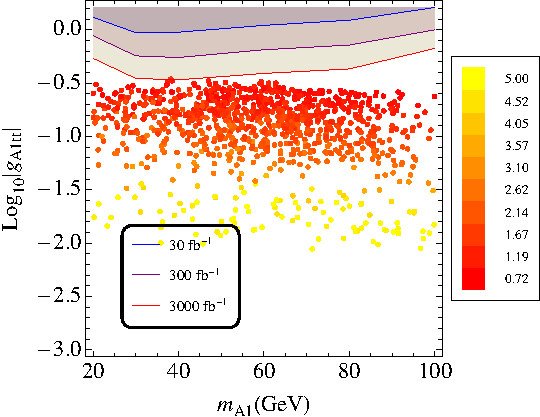
\includegraphics[width=0.45\textwidth]{Figures/pheno/plot_R1_NMSSM.pdf} &
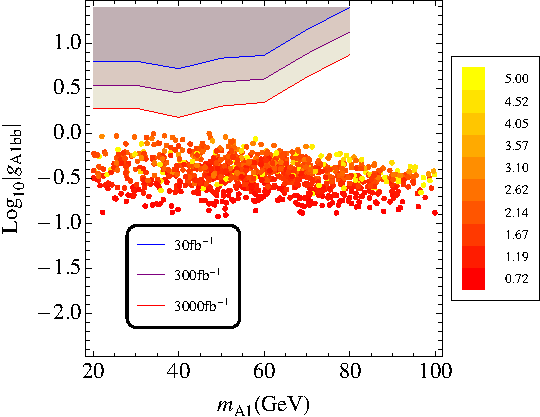
\includegraphics[width=0.45\textwidth]{Figures/pheno/plot_R3_NMSSM.pdf} \\
(a) & (b) \\
\end{tabular}
\caption{Sensitivity reach (at 95\% CL)  to the R-limit scenario in the NMSSM via the (a) $t\bar{t}A_1$ and (b) $b\bar{b} A_1$ channels. The scan is over all
  parameters, in the ranges $0.1 \leq \lambda \leq 0.6$, $0.1 \leq
  \kappa \leq 0.6$, $-7 \leq A_\lambda \leq 7$~GeV, $-7 \leq A_\kappa \leq 0$~GeV,
  $0.1 \leq \tan \beta \leq 5$, and $100 \leq \mu \leq 500$~GeV.  We
  have assumed soft squark masses of 2 TeV, slepton masses of 200 GeV,
  $A_{u,d,e} = -3.5$ TeV, and bino, wino and gluino masses of
  100, 200, and 2000 GeV, respectively. The hue of the scatter points represents the correspondent $\tan\beta$ values.}
\label{fig:reach_RS} 
\end{center}
\end{figure}


\item PQ-limit: $\frac{\kappa}{\lambda} \to 0$, $A_\kappa \to 0$, where the theory is approximately invariant under the transformation 
\begin{eqnarray}
H_u \to H_u \exp(i \phi_{\rm PQ}), \ \ H_d \to H_d \exp(i \phi_{\rm PQ}), \ \ S \to S \exp(-2i \phi_{\rm PQ}), 
\end{eqnarray}
and the tree-level mass of the PQ pseudo-Goldstone boson $A_1$ are given given by  
\begin{eqnarray}
m_{A_1} = - \frac{3 \kappa A_\kappa \mu}{\lambda}.
\end{eqnarray}
This scenario has been proposed as a supersymmetric benchmark for sub-electroweak scale (singlino-like) DM~\cite{Draper:2010ew}, since its lightest neutralino is generically singlino-like and lighter than the electroweak scale. Particularly, in this scenario $A_1$ can serve as the mediator for  DM annihilation into a bottom quark pair and explain the diffuse gamma-ray excess from the Galactic Centre~\cite{Huang:2014cla,Cheung:2014lqa}. In this limit, the tree-level couplings of $A_1$ with the top and bottom quarks are given by 
\begin{eqnarray}
y_{A_1 tt} = \frac{\lambda v \cos^2 \beta}{\mu}, \ \ y_{A_1 bb} = \frac{\lambda v \sin^2 \beta}{\mu},
\end{eqnarray}
and so smaller by a factor of two than the corresponding couplings in the R-limit. Furthermore, a smaller $\lambda$ is favoured in this limit and a relatively large $\tan\beta$ is needed to generate a mass of 125 GeV for the SM-like Higgs boson. Therefore, the coupling $y_{A_1 tt}$ tends to be smaller than in the R-limit scenario. 
The resulting values for the $y_{A_1tt}$ and $y_{A_1bb}$ couplings are compared to the expected collider bounds in Fig.~\ref{fig:reach_RS}(b).
For most of the points, the magnitude of $y_{A_1 tt}$ is below 0.1, which renders this scenario extremely difficult to probe at the using the $t\bar tA_1$ channel.\footnote{For alternative way to probing this scenario, using exotic Higgs decays, see e.g. Ref.~\cite{Huang:2013ima,Huang:2014cla,Butter:2015fqa}.}
 
\begin{figure}[htbp]
\begin{center}
\begin{tabular}{cc}
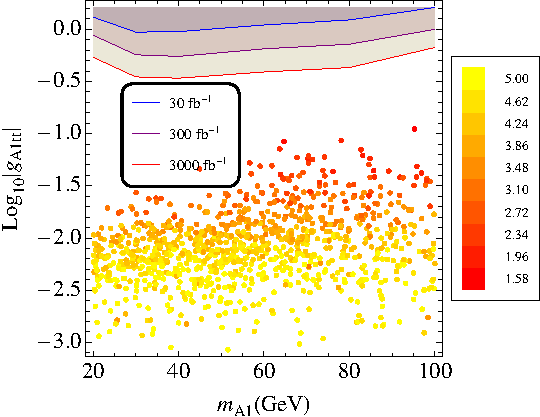
\includegraphics[width=0.45\textwidth]{Figures/pheno/plot_PQ1_NMSSM.pdf} &
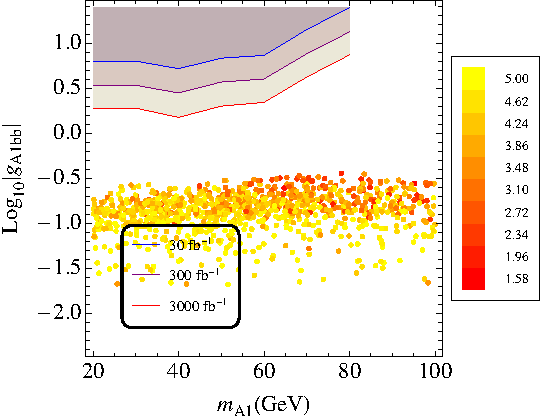
\includegraphics[width=0.45\textwidth]{Figures/pheno/plot_PQ3_NMSSM.pdf} \\
(a) & (b) \\
\end{tabular}
\caption{Sensitivity reach (at 95\% CL)  to the PQ-limit scenario in the NMSSM via the (a) $t\bar{t}A_1$ and (b) $b\bar{b} A_1$ channels. The scan is over all
  parameters, in the ranges $0.06 \leq \lambda \leq 0.6$, $5 \leq
  \kappa / \lambda \leq 100$, $|\varepsilon'| = \left| A_\lambda/\mu \tan\beta -1\right| \leq 0.25$, $-100 \leq A_\kappa \leq 0$~GeV,
  $0.1 \leq \tan \beta \leq 5$, and $100 \leq \mu \leq 500$~GeV.  We
  have assumed soft squark masses of 2 TeV, slepton masses of 200 GeV,
  $A_{u,d,e} = 3.5$ TeV, and bino, wino and gluino masses of
  100, 200, and 2000 GeV, respectively. The hue of the scatter points represents the correspondent $\tan\beta$ values.}
\label{fig:reach_PQ} 
\end{center}
\end{figure}

\end{enumerate}

Finally, we stress that the $b\bar b A_1$ channel doesn't help much in probing the R- and PQ-limit scenarios. The sensitivities of both searches are suppressed by the mixture with the singlet. Even worse, the mixing is approximately $\tan\beta$ enhanced, further suppressing the sensitivity of the $b\bar b A_1$ in probing the large $\tan\beta$ region in both scenarios.

